%!TeX root = ../Asq.tex
\begin{frame}[fragile]{Сервер (транслятор)}%
  Транслятор поддерживает обычные и агрегатные функции, а также стандартные секции SQL:
  \texttt{SELECT}, \texttt{FROM}, \texttt{WHERE}, \texttt{GROUP BY}, \texttt{HAVING} и \texttt{ORDER BY}.
  Возможна работа как с одной, так и несколькими таблицами (\texttt{JOIN}).

  Тестирование проводилось на одной из стандартных схем Oracle "--- HR.
  \begin{center}%
    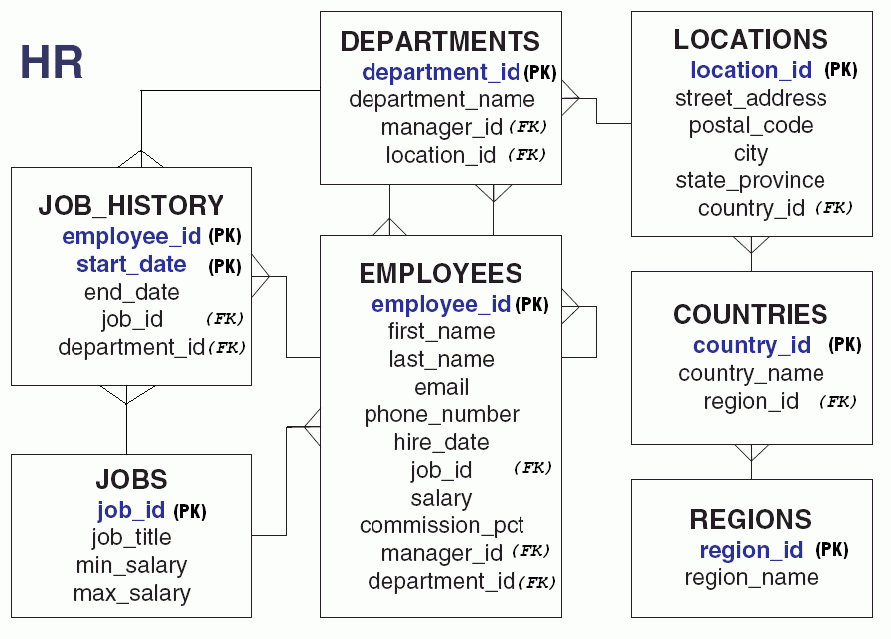
\includegraphics[width=0.4\textwidth]{img/scheme.png}
  \end{center}

\end{frame}
